\documentclass[
11pt, % The default document font size, options: 10pt, 11pt, 12pt
%codirector, % Uncomment to add a codirector to the title page
]{charter} 

% paquetes de JIT
\usepackage{makecell}
\usepackage{multirow, multicol}
\usepackage{longtable}
\usepackage{pgfgantt}
\usepackage{pdflscape}


% El títulos de la memoria, se usa en la carátula y se puede usar el cualquier lugar del documento con el comando \ttitle
\titulo{Desarrollo de una herramienta predictiva de la potencia límite de canal de la Central Nuclear Atucha II entrenada con simulaciones de código de subcanales} 

% Nombre del posgrado, se usa en la carátula y se puede usar el cualquier lugar del documento con el comando \degreename
%\posgrado{Carrera de Especialización en Sistemas Embebidos} 
%\posgrado{Carrera de Especialización en Internet de las Cosas} 
\posgrado{Carrera de Especialización en Inteligencia Artificial}
%\posgrado{Maestría en Sistemas Embebidos} 
%\posgrado{Maestría en Internet de las cosas}

% Tu nombre, se puede usar el cualquier lugar del documento con el comando \authorname
% IMPORTANTE: no omitir titulaciones ni tildación en los nombres, también se recomienda escribir los nombres completos (tal cual los tienen en su documento)
\autor{Ing. Juan Ignacio Teich}

% El nombre del director y co-director, se puede usar el cualquier lugar del documento con el comando \supname y \cosupname y \pertesupname y \pertecosupname
\director{Mgt. Ing. Martín Sebastián Silva}
\pertenenciaDirector{Nucleoeléctrica Argentina S.A.} 
\codirector{} % para que aparezca en la portada se debe descomentar la opción codirector en los parámetros de documentclass
\pertenenciaCoDirector{FIUBA}

% Nombre del cliente, quien va a aprobar los resultados del proyecto, se puede usar con el comando \clientename y \empclientename
\cliente{Departamento de Diseño Termohidráulico}
\empresaCliente{Nucleoeléctrica Argentina S.A.}
 
\fechaINICIO{3 de marzo de 2026}		%Fecha de inicio de la cursada de GdP \fechaInicioName
\fechaFINALPlan{21 de abril de 2026} 	%Fecha de final de cursada de GdP
\fechaFINALTrabajo{diciembre de 2026}	%Fecha de defensa pública del trabajo final

\newcommand{\CNA}{Central Nuclear Atucha II}

\begin{document}

\maketitle
\thispagestyle{empty}
\pagebreak


\thispagestyle{empty}
{\setlength{\parskip}{0pt}
\tableofcontents{}
}
\pagebreak


\section*{Registros de cambios}
\label{sec:registro}


\begin{table}[ht]
\label{tab:registro}
\centering
\begin{tabularx}{\linewidth}{@{}|c|X|c|@{}}
\hline
\rowcolor[HTML]{C0C0C0} 
Revisión & \multicolumn{1}{c|}{\cellcolor[HTML]{C0C0C0}Detalles de los cambios realizados} & Fecha      \\ \hline
0      & Creación del documento                                 &\fechaInicioName \\ \hline
1      & Se completa hasta el punto 5 inclusive                & 15 de marzo de 2026 \\ \hline
2      & Se completa hasta el punto 9 inclusive                & 22 de marzo de 2026 \\ \hline
3      & Se completa hasta el punto 12 inclusive               & 30 de marzo de 2026 \\ \hline
4      & Se completa hasta el punto 15 inclusive               & 4 de abril de 2026 \\ \hline
5      & Se corrigen comentarios sobre versión 4               & 11 de abril de 2026 \\ \hline
%		  Se puede agregar algo más \newline
%		  En distintas líneas \newline
%		  Así                                                    & {día} de {mes} de 202X \\ \hline
%3      & Se completa hasta el punto 12 inclusive                & {día} de {mes} de 202X \\ \hline
%4      & Se completa el plan	                                 & {día} de {mes} de 202X \\ \hline

% Si hay más correcciones pasada la versión 4 también se deben especificar acá

\end{tabularx}
\end{table}

\pagebreak



\section*{Acta de constitución del proyecto}
\label{sec:acta}

\begin{flushright}
Buenos Aires, \fechaInicioName
\end{flushright}

\vspace{2cm}

Por medio de la presente se acuerda con el \authorname{} que su Trabajo Final de la \degreename{} se titulará ``\ttitle'' y consistirá en la implementación de un modelo de aprendizaje profundo para cálculo de potencia límite de canal. El trabajo tendrá un presupuesto preliminar estimado de 600 horas y un costo estimado de \$6.250.000,00, con fecha de inicio el \fechaInicioName{} y fecha de presentación pública en \fechaFinalName{}.

Se adjunta a esta acta la planificación inicial.

\vfill

% Esta parte se construye sola con la información que hayan cargado en el preámbulo del documento y no debe modificarla
\begin{table}[ht]
\centering
\begin{tabular}{ccc}
\begin{tabular}[c]{@{}c@{}}Dr. Ing. Ariel Lutenberg \\ Director posgrado FIUBA\end{tabular} & \hspace{2cm} & \begin{tabular}[c]{@{}c@{}}\clientename \\ \empclientename \end{tabular} \vspace{2.5cm} \\ 
\multicolumn{3}{c}{\begin{tabular}[c]{@{}c@{}} \supname \\ Director del Trabajo Final\end{tabular}} \vspace{2.5cm} \\
\end{tabular}
\end{table}




% \section{1. Descripción técnica-conceptual del proyecto a realizar}
\section{Descripción técnica-conceptual del proyecto a realizar}
\label{sec:descripcion}

Dentro de las tareas necesarias para el funcionamiento de la \CNA{} (CNA-II) se tiene la determinación de la estrategia de recambio de combustibles. Los combustibles de la Central son compuestos por Uranio Natural, los cuales son recambiados por nuevos o reordenados dentro del propio reactor durante la operación para garantizar un correcto perfil de potencia en el reactor. El desarrollo de la estrategia en sí es parte de los cálculos neutrónicos del Departamento de Física del Reactor, pero una parte de este proceso es el cálculo de las potencias límites de canal (PLC) derivadas de las potencias de los elementos combustibles. Este cálculo es responsabilidad del \clientename{}, cliente del presente trabajo.

Las PLC tienen dos criterios por los cuales se calculan: margen a la desviación de la ebullición nucleada (Departure from Nucleate Boiling Ratio o DNBR), y por vacío (porcentaje de vapor en el fluido a la salida). El DNBR es un margen establecido en el diseño termohidráulico del reactor que tienen en cuenta las distintas incertidumbres que se tienen en el cálculo del DNB (desviación de la ebullición nucleada), y en el caso de la zona hidráulica 5 de CNA-II tiene un valor de $1.89$. El límite por vacío estipula que el fluido a la salida de los canales refrigerantes no debe tener más de un $25\%$ de vacío, por cuestiones de preservación mecánica de los canales refrigerantes. De estos dos criterios se elige aquel que tenga un menor valor de potencia como la potencia límite de canal.

Actualmente, el cálculo de las PLC se realiza por medio del software COBRA-3CP, un código de subcanales estándar de la industria nuclear, que fue modificado por la empresa INVAP para ajustarse a la geometría de diseño de los elementos combustibles del reactor de CNA-II. Los datos de entrada para el cálculo con COBRA son:
\begin{itemize}
  \item Perfil de potencia axial global.
  \item Perfil de potencia radial para cada barra combustible.
  \item Condiciones del agua pesada a la entrada del canal refrigerante (caudal, presión y temperatura).
\end{itemize}
Estos parámetros cambian para cada estado del reactor, y en cada estado del reactor cambian para cada uno de los 451 canales refrigerantes. Entonces se tienen 451 cálculos a realizar por cada estado del reactor en una estrategia de recambio de combustibles, las cuales pueden tener entre 4000 y 10000 estados, llevando la cantidad de casos a simular por COBRA por sobre los 4 millones en algunos casos. Esto implica periodos de cálculo muy extensos, y además se debe tener la capacidad de almacenamiento de las salidas del código para su post procesamiento, o realizar post procesamiento en línea con las dificultades que esto conlleva. 

Lo único que termina interesando son los casos que predicen la menor PLC para cada canal refrigerante, por lo que gran parte de la salida entregada por COBRA no es de interés. Es sobre este punto que se plantea desarrollar una herramienta que permita estimar la PLC de manera más rápida y eficiente en almacenamiento, para poder obtener los peores casos para cada canal refrigerante y luego validar con COBRA el resultado de PLC en ellos (por razones normativas).

Se propone implementar una red neuronal entrenada a partir de las simulaciones realizadas con COBRA para casos de estrategia de combustible, es decir, con el reactor en condiciones nominales. Se evaluará la implementación de variantes de redes neuronales tradicionales, como redes neuronales informadas por física, aplicando las ecuaciones de balance de masa, energía y de cantidad de movimiento, así como también las ecuaciones de subcanales que tiene incorporadas COBRA.

Es de interés también obtener conocimiento sobre como las distintas formas de los perfiles de potencia impactan en las PLC, por lo que se realizará un estudio sobre ello por medio de embeddings que concentren las características principales de los perfiles.

En la Figura \ref{fig:diag_bloques} se tiene un diagrama de bloques del proceso de cálculo actual y del propuesto a desarrollar en este trabajo.

\begin{figure}[htpb]
  \centering
  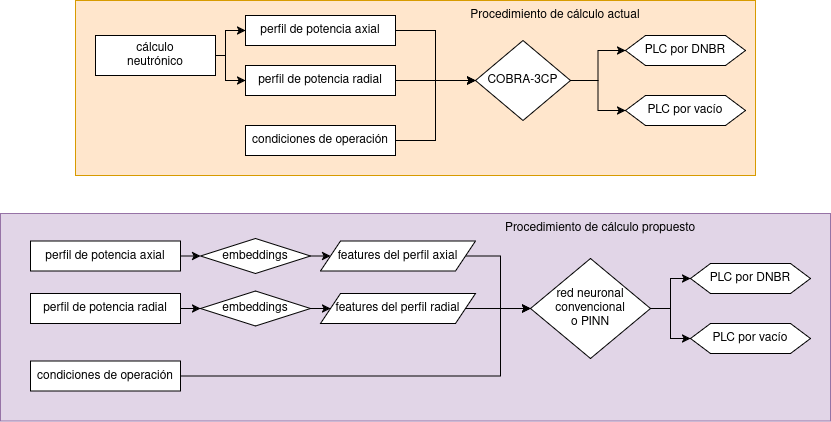
\includegraphics[width=\textwidth]{Figuras/diag_bloques_CEIA_TPF.png}
  \caption{Diagrama de bloques de método de cálculo actual y propuesto.} \label{fig:diag_bloques}
\end{figure}

% \section{2. Identificación y análisis de los interesados}
\section{Identificación y análisis de los interesados}
\label{sec:interesados}

\begin{table}[ht]
\caption{Identificación de los interesados}
\label{tab:interesados}
\begin{tabularx}{\linewidth}{@{}|l|X|X|l|@{}}
\hline
\rowcolor[HTML]{C0C0C0} 
Rol           & Nombre y Apellido & Organización 	& Puesto 	\\ \hline
Cliente       & \clientename      &\empclientename	& -       	\\ \hline
Responsable   & \authorname       & FIUBA        	& Alumno 	\\ \hline
Orientador    & \supname	      & \pertesupname 	& Director del Trabajo Final \\ \hline
Usuario       & \clientename      &\empclientename	& -       	\\ \hline
\end{tabularx}
\end{table}

\begin{itemize}
  \item Orientador: el Mgt. Ing. Martín Silva es el Jefe del \clientename{}, experto dentro de la industria nuclear con 20 años de experiencia en la Gerencia de Análisis de Seguridad y Diseño del Núcleo de Nucleoeléctrica Argentina S.A., y va a ayudar en la definición del alcance y en el desarrollo de la herramienta predictiva.
\end{itemize}

% \section{3. Propósito del proyecto}
\section{Propósito del proyecto}
\label{sec:proposito}

Desarrollar un método de cálculo superador en cuanto a requerimientos de recursos computacionales, tiempos y logística computacional. Esto implicaría una disminución en la carga de trabajo del \clientename{}, permitiendo abocar más recursos y tiempos a otras tareas. Además, adquirir conocimiento respecto de la relación entre las variables de entrada y las PLC es algo deseado por el Departamento.

% \section{4. Alcance del proyecto}
\section{Alcance del proyecto}
\label{sec:alcance}

El proyecto incluye:
\begin{itemize}
  \item Desarrollo de un modelo de aprendizaje profundo que pueda replicar con error razonable los resultados que entrega el software COBRA-3CP, dentro de las condiciones de operación nominal de la \CNA{}.
  \item Desarrollo de un flujo de trabajo para cálculo de las PLC con el modelo como centro.
  \item Análisis de embeddings y características principales de los perfiles de potencia axial y radial, y su influencia en el valor final de PLC.
\end{itemize}

Se encuentran fuera del alcance del proyecto:
\begin{itemize}
  \item Entrenamiento y evaluación del modelo en condiciones alejadas de la nominal.
  \item Implementación del modelo dentro de otros códigos pertenecientes al \clientename{}.
  \item Implementación desde cero del modelo de aprendizaje profundo.
\end{itemize}

% \section{5. Supuestos del proyecto}
\section{Supuestos del proyecto}
\label{sec:supuestos}

Para el desarrollo del presente proyecto se supone que: 
\begin{itemize}
  \item \textbf{Supuesto 1:} el Alumno dispondrá de tiempo similar cada semana para el desarrollo del trabajo, con imprevistos que impidan la normal dedicación poco frecuentes. Está planeado dentro de las tareas laborales la realización de este trabajo.
  \item \textbf{Supuesto 2:} se contará con disponibilidad de datos de simulaciones ya realizadas con COBRA, así como también la realización de nuevas simulaciones si fueran necesarias.
  \item \textbf{Supuesto 3:} las herramientas disponibles online para implementación de modelos de aprendizaje profundo son adecuadas, confiables y eficientes para su uso en este trabajo, por ejemplo: \textit{scikit-learn}, \textit{pytorch}, \textit{numpy}, etc.
  \item \textbf{Supuesto 4:} se tendrá acceso a capacidad de cómputo, ya sea por medios locales del \clientename{} o del Alumno, o por medios en la nube como \textit{Google Colab}.
\end{itemize}

% \section{6. Product Backlog}
\section{Product Backlog}
\label{sec:backlog}

A continuación se describen las épicas e historias de usuario de cada épica:

\begin{itemize}
  \item \textbf{Épica 1: adquisición de datos}
    \begin{itemize}
      \item HU1: como Responsable, quiero determinar, en conjunto con el Director, el set de datos a adquirir, determinando qué casos ya están simulados y aquellos que deben ser simulados, para poder procesar los datos de forma acorde a su posterior utilización. Story points: 5 (tiempo: 1, dificultad: 3, incerteza: 1).
      \item HU2: como Responsable, quiero simular los casos faltantes, para completar el set de datos de entrenamiento. Story points: 3 (tiempo: 1, dificultad: 1, incerteza: 1).
      \item HU3: como Responsable, quiero desarrollar la herramienta para procesar archivos OUTPUT de COBRA, para armar el set de datos. Story points: 8 (tiempo: 4, dificultad: 3, incerteza: 1).
      %\item HU4: como Usuario final, quiero que la forma de ingreso de los datos esté definida y sea simple de implementar, para poder utilizar la herramienta de forma sencilla.
    \end{itemize}
  \item \textbf{Épica 2: desarrollo de modelo de red neuronal convencional}
    \begin{itemize}
      \item HU4: como Responsable, quiero probar distintas arquitecturas de red neuronal en base a los datos de simulaciones de COBRA, para obtener finalmente un modelo de red neuronal base funcional entregable. Story points: 21 (tiempo: 9, dificultad: 9, incerteza: 3).
      \item HU5: como Usuario final, quiero tener un modelo básico con documentación de uso y métricas, para poder replicar los resultados que se obtienen con COBRA de forma más rápida y eficiente. Story points: 5 (tiempo: 1, dificultad: 3, incerteza: 3).
    \end{itemize}
  \item \textbf{Épica 3: análisis de embeddings y feature engineering para perfiles de potencia axiales y radiales}
    \begin{itemize}
      \item HU6: como Reponsable, quiero implementar feature engineering y embeddings sobre los datos de entrada, para buscar mejorar las capacidades predictivas de la red neuronal base. Story points: 13 (tiempo: 3, dificultad: 7, incerteza: 3).
      \item HU7: como Cliente, quiero obtener figuras de mérito de los perfiles de potencia y combinación de otras variables, para mejorar la propuesta de estrategias de recambio de combustibles. Story points: 13 (tiempo: 3, dificultad: 7, incerteza: 3).
    \end{itemize}
  \item \textbf{Épica 4: implementación de red neuronal informada por física}
    \begin{itemize}
      \item HU8: como Responsable, quiero investigar y estudiar sobre redes neuronales informadas por física, para poder implementar dicho modelo. Story points: 21 (tiempo: 9, dificultad: 9, incerteza: 3).
      \item HU9: como Cliente, quiero evaluar el impacto de utilizar redes neuronales informadas por física, para garantizar predicciones físicamente válidas. Story points: 13 (tiempo: 3, dificultad: 5, incerteza: 5).
    \end{itemize}
\end{itemize}

% En el Cuadro \ref{tab:story_points} se tienen los story points y prioridad de cada historia de usuario, que están basados en el criterio establecido por el Cuadro \ref{tab:criterio_story_points}.

% \begin{table}[hbt]
%   \centering
%   \begin{tabular}{c|c|c|c|c|c}
%     \hline
%     Nro. HU & \thead{Tiempo\\ requerido} & \thead{Dificultad/complejidad\\ de la tarea} & \thead{Incerteza \\y riesgo} & Story points & Prioridad \\ \hline
%     1 & Bajo & Media & Bajo & 5 & Alta\\ \hline
%     2 & Bajo & Bajo & Bajo & 3 & Media\\ \hline
%     3 & Medio & Medio & Bajo & 8 & Alta\\ \hline \hline
%     4 & Alto & Alto & Medio & 21 & Alta\\ \hline
%     5 & Bajo & Medio & Medio & 5 & Alta\\ \hline \hline
%     6 & Medio & Alta & Alta & 13 & Medio\\ \hline
%     7 & Medio & Alta & Alta & 13 & Baja\\ \hline \hline
%     8 & Alta & Alta & Alta & 21 & Media\\ \hline
%     9 & Media & Media & Alta & 8 & Media\\ \hline
    
%   \end{tabular}
%   \caption{Story points y prioridad de las historias de usuario.}
%   \label{tab:story_points}
% \end{table}

% \begin{table}[hbt]
%   \centering
%   \begin{tabular}{c|c|c|c}
%     \hline
%     \thead{Tiempo\\ requerido} & \thead{Dificultad/complejidad\\ de la tarea} & \thead{Incerteza \\y riesgo} & Story points\\ \hline
%     Bajo        & Bajo        & Bajo        & 3\\ \hline 
%     Bajo        & Medio       & Bajo-Medio  & 5\\ \hline 
%     Medio       & Medio       & Medio       & 8\\ \hline 
%     Medio       & Alto        & Medio-Alto  & 13\\ \hline 
%     Alto        & Alto        & Medio-Alto  & 21\\ \hline 
%   \end{tabular}
%   \caption{Criterio de valor de story points.}
%   \label{tab:criterio_story_points}
% \end{table}

% \section{7. Criterios de aceptación de historias de usuario}
\section{Criterios de aceptación de historias de usuario}
\label{sec:criteriosAceptacion}

A continuación se establecen los criterios de aceptación de cada historia de usuario:

\begin{itemize}
  \item \textbf{Épica 1: adquisición de datos}
    \begin{itemize}
      \item HU1 - determinación del set de datos:
        \begin{itemize}
          % \item Realizar la búsqueda de datos disponible en el almacenamiento de la Gerencia.
          \item Se dispone de un inventario documentado de todos los datos de simulaciones disponibles.
          % \item Compilación de datos en un único directorio, con codificación de cada uno de forma clara.
          \item Se tiene un documento con los casos ya simulados y aquellos que es necesario simular.
          % \item Listado de datos disponibles y datos a simular.
        \end{itemize}
      \item HU2 - simulación de datos faltantes:
        \begin{itemize}
          \item Se tiene un script para generar los inputs de los casos faltantes y simularlos.
          % \item Simulación de todos los datos faltantes establecidos previamente con COBRA-3CP.
          \item Se dispone de un inventario con todos los casos necesarios.
          % \item Almacenado de los archivos OUTPUT, siguiendo reglas de codificación previamente establecidas.
        \end{itemize}
      \item HU3 - herramienta de procesamiento de archivos OUTPUT:
        \begin{itemize}
          \item Se tiene una herramienta que permita procesar en batch archivos OUTPUT, obteniendo un único archivo de fácil importación luego (p.e.: .csv, .json, .parquet, etc.).
          \item Se dispone de todos los datos almacenados en un único archivo.
          % \item Procesado de todos los datos almacenados y guardado en un archivo único (p.e.: .parquet).
        \end{itemize}
    \end{itemize}
  \item \textbf{Épica 2: desarrollo de modelo de red neuronal convencional}
    \begin{itemize}
      \item HU4 - prueba de arquitectura de red neuronal:
        \begin{itemize}
          \item Se tiene una Jupyter Notebook con todas las pruebas de hiperparámetros, funciones de activación, etc. probadas, con las métricas pertinentes graficadas.
          % \item Realizar y documentar pruebas de hiperparámetros, funciones de activación, etc. teniendo en cuenta métricas y análisis de sobreajuste.
          % \item Obtener relación entre hiperparámetros, funciones de activación, etc. y precisión.
          % \item Análisis  posible sobreajuste del modelo.
          \item Se tiene un modelo con la arquitectura óptima según la Notebook anterior.
          % \item Determinar la arquitectura óptima para el problema en cuestión.
        \end{itemize}
      \item HU5 - modelo básico documentado:
        \begin{itemize}
          \item Se tiene un repositorio de github documentado del modelo final en python.
          \item Se tiene un documento con el detalle de la arquitectura del modelo y sus métricas.
        \end{itemize}
    \end{itemize}
  \item \textbf{Épica 3: análisis de embeddings y feature engineering para perfiles de potencia axiales y radiales}
    \begin{itemize}
      \item HU6 - feature engineering y embeddings:
        \begin{itemize}
          \item Se tiene una Jupyter Notebook con una implementación básica de embeddings para los perfiles de potencia.
          % \item Implementación de embeddings para los perfiles de potencia.
          \item Se tiene una Jupyter Notebook con feature engineering, probando agregando y/o sacando features, analizando dependencia, etc.
          % \item Análisis de posible feature engineering: agregado de features que antes no se consideraban, descartado de features, análisis de dependencia, etc.
          \item Se dispone de una Jupytern Notebook con un modelo que implementa los embeddings y feature engineering, comparado con el modelo base de la HU5.
          % \item Definición de un modelo de red neuronal implementando lo anterior y comparación con modelo base.
        \end{itemize}
      \item HU7 - figuras de mérito:
        \begin{itemize}
          % \item Análisis de los embeddings una vez entrenados, en particular si representan características puntuales de los perfiles de potencia.
          \item Se tiene una Jupyter Notebook donde se analiza si los embeddings entrenados en la HU6 representan características puntuales de los perfiles de potencia.
          % \item Definición de figuras de mérito de los perfiles de potencia en base a los embeddings y feature engineering.
          \item Se tiene un documento donde se explican figuras de mérito de los perfiles de potencia en función de los embeddings y feature engineering realizados.
        \end{itemize}
    \end{itemize}
  \item \textbf{Épica 4: implementación de red neuronal informada por física}
    \begin{itemize}
      \item HU8 - estudio redes neuronales informadas por física:
        \begin{itemize}
          \item Se tiene aprobada la materia ``Redes Neuronales Informadas por Física" de la CEIA.
          % \item Estudio del estado del arte en papers y libros.
          % \item Estudio de herramientas pre-codificadas (paquetes de python).
          \item Se dispone de una Jupyter Notebook con implementación de casos simples de bibliografía.
        \end{itemize}
      \item HU9 - implementación redes neuronales informadas por física:
        \begin{itemize}
          \item Se tiene un documento con las ecuaciones a implementar en el modelo desarolladas.
          \item Se dispone de una Jupyter Notebook con una implementación de una red neuronal informada por física.
          \item Se tiene una Jupyter Notebook con el análisis de hiperparámetros y métricas de la PINN.
          \item Se tiene una Jupyter Notebook con un modelo de PINN, comparado con los modelos definidos en la HU5 y la HU6.
          % \item Definición de las ecuaciones a implementar en el modelo.
          % \item Implementación de la red neuronal informada por física.
          % \item Análisis de hiperparámetros y métricas.
          % \item Definición de modelo informado por física final y comparativa con modelos previos.
        \end{itemize}
    \end{itemize}
\end{itemize}

% \section{8. Fases de CRISP-DM}
\section{Fases de CRISP-DM}

\begin{enumerate}
  \item \textbf{Comprensión del negocio:}
    \begin{itemize}
      \item Objetivo: desarrollar una herramienta basada en aprendizaje profundo para predecir las potencias límite de canal de CNA-II con un menor costo computacional al método actual con COBRA-3CP.
      \item Impacto: disminución del costo computacional, el tiempo de cálculo y los requerimientos de almacenamiento para simulaciones de estrategias de recambio de combustibles.
      \item Métricas: tiempo para predicción sobre una gran cantidad de casos contra tiempo de simulación con COBRA-3CP, error relativo y absoluto frente a COBRA-3CP.
    \end{itemize}
  \item \textbf{Comprensión de los datos:}
    \begin{itemize}
      \item Tipos de datos: archivos de OUTPUT de COBRA-3CP.
      \item Fuentes de datos: simulaciones con COBRA-3CP.
      \item Cantidad de datos: del orden de decenas de miles.
      \item Calidad de datos: los datos deben ser procesados desde los archivos de texto a valores.
    \end{itemize}
  \item \textbf{Preparación de los datos:}
    \begin{itemize}
      \item Transformaciones: parseo de los archivos de OUTPUT para obtener la información requerida.
      % \item Características clave:
    \end{itemize}
  \item \textbf{Modelado:}
    \begin{itemize}
        \item Modelo de aprendizaje profundo: arquitectura de red neuronal tradicional, uso de embeddings, arquitectura de red neuronal informada por física.
    \end{itemize}
  \item \textbf{Evaluación del modelo:}
    \begin{itemize}
        \item Métricas: error relativo y absoluto en predicción de potencia límite de canal frente a COBRA-3CP, error relativo y absoluto en otras variables de interés de la salida de COBRA, tiempo para ejecutar una predicción.
    \end{itemize}
\end{enumerate}

\newpage
% \section{9. Desglose del trabajo en tareas}
\section{Desglose del trabajo en tareas}
\label{sec:wbs}

A continuación, en el Cuadro \ref{tab:tareas_por_hu}, se describen las tareas necesarias de cada historia de usuario.

\begin{longtable}{|p{4cm}|p{6cm}|c|c|}
\caption{Desglose de tareas por historia de usuario.}
\label{tab:tareas_por_hu} \\
\hline
\rowcolor[HTML]{C0C0C0}
Historia de usuario & Tarea técnica & Estimación & Prioridad \\ \hline \endfirsthead
\multicolumn{4}{c}{{Continuación de anterior página}} \\
\rowcolor[HTML]{C0C0C0}
Historia de usuario & Tarea técnica & Estimación & Prioridad \\ \hline
\endhead
\hline \multicolumn{4}{|r|}{{Continúa en próxima página}} \\ \hline
\endfoot
\hline \hline
\endlastfoot

\multirow{3}{4cm}{HU1 - Determinación del set de datos}  
  & 1.1: Recopilación de datos de simulaciones de COBRA para estrategias de combustibles. & 9 h & Alta \\* \cline{2-4}
  \nopagebreak & 1.2: Documentación de casos contemplados por las simulaciones ya hechas y cataloguización de los mismos. & 7 h & Alta \\* \cline{2-4}
  & 1.3: Definición de datos de simulaciones faltantes. & 3 h & Alta \\ \hline

\multirow{4}{4cm}{HU2 - Simulación de datos faltantes}  
  & 2.1: Desarrollo de herramienta para automatización de generación de INPUTS. & 10 h & Media \\* \cline{2-4}
  & 2.2: Armado de INPUTS sobre casos faltantes. & 8 h & Media \\* \cline{2-4}
  & 2.3: Simulación de casos faltantes. & 6 h & Media \\* \cline{2-4}
  & 2.4: Almacenado y cataloguización de salidas de las simulaciones. & 3 h & Media \\ \hline

\multirow{2}{4cm}{HU3 - Herramienta de procesamiento de archivos de OUTPUT}  
  & 3.1: Desarrollo de herramienta para procesamiento de archivos de OUTPUT. & 12 h & Alta \\* \cline{2-4}
  & 3.2: Procesado de archivos de OUTPUT. & 4 h & Alta \\ \hline

\multirow{4}{4cm}{HU4 - Prueba de arquitectura de red neuronal} 
  & 4.1: Armado de estructura base sobre la que realizar pruebas. & 8 h & Alta \\* \cline{2-4}   
  & 4.2: Realizado de pruebas de funciones de activación de la red neuronal. & 8 h & Alta \\* \cline{2-4}
  & 4.3: Realizado de pruebas de hiperparámetros de la red neuronal. & 8 h & Alta \\* \cline{2-4}
  & 4.4: Graficado de métricas y comparativa entre arquitecturas. & 6 h & Alta \\* \cline{2-4}
  & 4.5: Definición de arquitectura final. & 4 h & Alta \\ \hline

\multirow{3}{4cm}{HU5 - Modelo básico documentado}  
  & 5.1: Documentado de resultados de pruebas de arquitectura. & 6 h & Alta \\* \cline{2-4}
  & 5.2: Documentado de arquitectura final de red neuronal. & 6 h & Alta \\* \cline{2-4}
  & 5.3: Armado de versión entrenada en github del modelo. & 3 h & Alta \\ \hline

\pagebreak

\multirow{8}{4cm}{HU6 - Feature engineering y embeddings}  
  & 6.1: Definición de nuevas features derivadas para probar su efecto. & 12 h & Alta \\* \cline{2-4}
  & 6.2: Pruebas de nuevas features. & 12 h & Alta \\* \cline{2-4}
  & 6.3: Armado de estructura base para entrenar embeddings. & 8 h & Alta \\* \cline{2-4}
  & 6.4: Prueba de entrenamientos de embeddings de los perfiles de potencia axial. & 8 h & Alta \\* \cline{2-4}
  & 6.5: Prueba de entrenamientos de embeddings de los perfiles de potencia radial. & 8 h & Alta \\* \cline{2-4}
  & 6.6: Análisis de diferencias en los perfiles según valores de embeddings. & 6 h & Alta \\* \cline{2-4}
  & 6.7: Prueba de modelo con embeddings y nuevas features. & 8 h & Alta \\* \cline{2-4}
  & 6.8: Definición de nuevo modelo incorporando embeddings y nuevas features. & 6 h & Alta \\* \cline{2-4}
  & 6.9: Comparativa de performance contra modelo base de red neuronal. & 4 h & Alta \\ \hline

\multirow{2}{4cm}{HU7 - Figuras de mérito}  
  & 7.1: Análisis de figuras de mérito en función de los embeddings entrenados y su relación con las PLC. & 12 h & Baja \\* \cline{2-4}
  & 7.2: Documentación de efecto de las figuras de mérito en las PLC. & 4 h & Baja \\ \hline

\multirow{3}{4cm}{HU8 - Estudio de redes neuronales informadas por física}  
  & 8.1: Cursado de materia ``Redes Neuronales Informadas por Física". & 48 h & Media \\* \cline{2-4}
  & 8.2: Lectura del estado del arte. & 12 h & Media \\* \cline{2-4}
  & 8.3: Aplicación de ejemplos básicos de redes neuronales informadas por física. & 12 h & Media \\ \hline

\pagebreak

\multirow{7}{4cm}{HU9 - Implementación de redes neuronales informadas por física}  
  & 9.1: Recopilación de ecuaciones de balance utilizadas por COBRA. & 12 h & Media \\* \cline{2-4}
  & 9.2: Definición de las ecuaciones a aplicar en el modelo. & 8 h & Media \\* \cline{2-4}
  & 9.3: Armado de modelo base de red neuronal informada por física con las ecuaciones definidas. & 8 h & Media \\* \cline{2-4}
  & 9.4: Análisis de arquitecturas. & 8 h & Media \\* \cline{2-4}
  & 9.5: Análisis de hiperparámetros. & 8 h & Media \\* \cline{2-4}
  & 9.6: Definición de red neuronal informada por física final. & 4 h & Media \\* \cline{2-4}
  & 9.7: Comparativa de performance contra modelos previamente desarrollados. & 4 h & Media \\* \cline{2-4}
  & 9.8: Documentación final de modelo final de red neuronal informada por física. & 4 h & Media \\ \hline
\end{longtable}


\newpage
% \section{10. Planificación de Sprints}
\section{Planificación de Sprints}

En el Cuadro \ref{tab:tareas} se tiene la planificación de Sprints en función de las tareas definidas previamente.

\begin{longtable}{|l|l|p{3cm}|p{1cm}|p{2cm}|c|}
\caption{Planificación de Sprints.}
\label{tab:tareas} \\
\hline
\rowcolor[HTML]{C0C0C0}
Sprint & HU o fase & Tarea & Horas / SP & Responsable & \% Completado \\ \hline \endfirsthead
\multicolumn{6}{c}{{Continuación de anterior página}} \\
\rowcolor[HTML]{C0C0C0}
Sprint & HU o fase & Tarea & Horas / SP & Responsable & \% Completado \\ \hline
\endhead
\hline \multicolumn{6}{|r|}{{Continúa en próxima página}} \\ \hline
\endfoot
\hline \hline
\endlastfoot

\multirow{4}{*}{Sprint 0} 
 & Planificación & Def. alcance y cronograma & 10 h & Alumno y Director & 100\% \\ \cline{2-6} 
 & Planificación & Reuniones & 5 h & Alumno y Director & 100\% \\ \cline{2-6} 
 & Planificación & Ajuste Engregables & 6 h & Alumno y Director & 50\% \\ \cline{2-6} 
 & \multicolumn{5}{|c|}{Total: 21 h} \\ \hline \hline

\multirow{9}{*}{Sprint 1} 
 & HU1 & Tarea 1 & 9 h & Alumno y Director            & 0\% \\ \cline{2-6} 
 & HU1 & Tarea 2 & 7 h & Alumno                       & 0\% \\ \cline{2-6} 
 & HU1 & Tarea 3 & 3 h & Alumno y Director            & 0\% \\ \cline{2-6}
 & HU2 & Tarea 1 & 10 h & Alumno                       & 0\% \\ \cline{2-6} 
 & HU8 & Tarea 1 & 12 h & Alumno                       & 0\% \\ \cline{2-6}
 & Planificación & Reuniones & 6 h & Alumno y Director  & 0\% \\ \cline{2-6}
 & Escritura & Redacción memoria & 4 h & Alumno         & 0\% \\ \cline{2-6}
 & \multicolumn{5}{|c|}{Total: 51 h} \\ \hline \hline

\multirow{9}{*}{Sprint 2} 
 & HU2 & Tarea 2 & 8 h & Alumno                       & 0\% \\ \cline{2-6} 
 & HU2 & Tarea 3 & 6 h & Alumno                       & 0\% \\ \cline{2-6}
 & HU2 & Tarea 4 & 3 h & Alumno                       & 0\% \\ \cline{2-6}
 & HU3 & Tarea 1 & 12 h & Alumno                       & 0\% \\ \cline{2-6} 
 & HU8 & Tarea 1 & 12 h & Alumno                       & 0\% \\ \cline{2-6}
 & Planificación & Reuniones & 6 h & Alumno y Director  & 0\% \\ \cline{2-6}
 & Escritura & Redacción memoria & 4 h & Alumno         & 0\% \\ \cline{2-6}
 & \multicolumn{5}{|c|}{Total: 51 h} \\ \hline \hline

\multirow{8}{*}{Sprint 3} 
 & HU3 & Tarea 2 & 4 h & Alumno                       & 0\% \\ \cline{2-6} 
 & HU4 & Tarea 1 & 8 h & Alumno                       & 0\% \\ \cline{2-6} 
 & HU4 & Tarea 2 & 8 h & Alumno                       & 0\% \\ \cline{2-6} 
 & HU4 & Tarea 3 & 8 h & Alumno                       & 0\% \\ \cline{2-6} 
 & HU8 & Tarea 1 & 12 h & Alumno                      & 0\% \\ \cline{2-6}
 & Planificación & Reuniones & 6 h & Alumno y Director  & 0\% \\ \cline{2-6}
 & Escritura & Redacción memoria & 4 h & Alumno         & 0\% \\ \cline{2-6}
 & \multicolumn{5}{|c|}{Total: 50 h} \\ \hline \hline

\pagebreak

\multirow{10}{*}{Sprint 4} 
 & HU4 & Tarea 4 & 6 h & Alumno                       & 0\% \\ \cline{2-6} 
 & HU4 & Tarea 5 & 4 h & Alumno y Director            & 0\% \\ \cline{2-6}
 & HU5 & Tarea 1 & 6 h & Alumno                       & 0\% \\ \cline{2-6}
 & HU5 & Tarea 2 & 6 h & Alumno                       & 0\% \\ \cline{2-6} 
 & HU5 & Tarea 3 & 3 h & Alumno                       & 0\% \\ \cline{2-6} 
 & HU6 & Tarea 1 & 6 h & Alumno                       & 0\% \\ \cline{2-6}
 & HU8 & Tarea 1 & 12 h & Alumno                       & 0\% \\ \cline{2-6}
 & Planificación & Reuniones & 6 h & Alumno y Director  & 0\% \\ \cline{2-6}
 & Escritura & Redacción memoria & 8 h & Alumno         & 0\% \\ \cline{2-6}
 & \multicolumn{5}{|c|}{Total: 57 h} \\ \hline \hline

\multirow{7}{*}{Sprint 5} 
 & HU6 & Tarea 2 & 12 h & Alumno                       & 0\% \\ \cline{2-6} 
 & HU6 & Tarea 3 & 12 h & Alumno                       & 0\% \\ \cline{2-6} 
 & HU6 & Tarea 4 & 8 h & Alumno                       & 0\% \\ \cline{2-6} 
 & HU6 & Tarea 5 & 8 h & Alumno                       & 0\% \\ \cline{2-6} 
 & Planificación & Reuniones & 6 h & Alumno y Director  & 0\% \\ \cline{2-6}
 & Escritura & Redacción memoria & 8 h & Alumno         & 0\% \\ \cline{2-6}
 & \multicolumn{5}{|c|}{Total: 54 h} \\ \hline \hline

\multirow{9}{*}{Sprint 6} 
 & HU6 & Tarea 6 & 6 h & Alumno                       & 0\% \\ \cline{2-6} 
 & HU6 & Tarea 7 & 8 h & Alumno                       & 0\% \\ \cline{2-6} 
 & HU6 & Tarea 8 & 6 h & Alumno                       & 0\% \\ \cline{2-6} 
 & HU6 & Tarea 9 & 4 h & Alumno                       & 0\% \\ \cline{2-6} 
 & HU7 & Tarea 1 & 12 h & Alumno                       & 0\% \\ \cline{2-6} 
 & HU7 & Tarea 2 & 4 h & Alumno                       & 0\% \\ \cline{2-6} 
 & Planificación & Reuniones & 6 h & Alumno y Director  & 0\% \\ \cline{2-6}
 & Escritura & Redacción memoria & 20 h & Alumno         & 0\% \\ \cline{2-6}
 & \multicolumn{5}{|c|}{Total: 66 h} \\ \hline \hline

\multirow{6}{*}{Sprint 7} 
 & HU8 & Tarea 2 & 12 h & Alumno                       & 0\% \\ \cline{2-6} 
 & HU8 & Tarea 3 & 12 h & Alumno                       & 0\% \\ \cline{2-6} 
 & HU9 & Tarea 1 & 12 h & Alumno                       & 0\% \\ \cline{2-6} 
 & Planificación & Reuniones & 6 h & Alumno y Director  & 0\% \\ \cline{2-6}
 & Escritura & Redacción memoria & 20 h & Alumno         & 0\% \\ \cline{2-6}
 & \multicolumn{5}{|c|}{Total: 62 h} \\ \hline \hline

\pagebreak

\multirow{7}{*}{Sprint 8} 
 & HU9 & Tarea 2 & 8 h & Alumno                       & 0\% \\ \cline{2-6} 
 & HU9 & Tarea 3 & 8 h & Alumno                       & 0\% \\ \cline{2-6} 
 & HU9 & Tarea 4 & 8 h & Alumno                       & 0\% \\ \cline{2-6} 
 & HU9 & Tarea 5 & 8 h & Alumno                       & 0\% \\ \cline{2-6} 
 & Planificación & Reuniones & 6 h & Alumno y Director  & 0\% \\ \cline{2-6}
 & Escritura & Redacción memoria & 30 h & Alumno         & 0\% \\ \cline{2-6}
 & \multicolumn{5}{|c|}{Total: 68 h} \\ \hline \hline

\multirow{6}{*}{Sprint 9} 
 & HU9 & Tarea 6 & 4 h & Alumno                       & 0\% \\ \cline{2-6} 
 & HU9 & Tarea 7 & 4 h & Alumno                       & 0\% \\ \cline{2-6} 
 & HU9 & Tarea 8 & 4 h & Alumno                       & 0\% \\ \cline{2-6} 
 & Planificación & Reuniones & 6 h & Alumno y Director  & 0\% \\ \cline{2-6}
 & Escritura & Redacción memoria & 40 h & Alumno         & 0\% \\ \cline{2-6}
 & \multicolumn{5}{|c|}{Total: 58h} \\ \hline \hline

\multirow{4}{*}{Sprint 10} 
 & Planificación & Reuniones & 6 & Alumno y Director  & 0\% \\ \cline{2-6}
 & Escritura & Redacción memoria & 30 & Alumno         & 0\% \\ \cline{2-6}
 & Defensa & Preparación & 20 h & Alumno         & 0\% \\ \cline{2-6}
 & \multicolumn{5}{|c|}{Total: 56 h} \\ \hline \hline

\end{longtable}

% \section{11. Diagrama de Gantt (sprints)}
\section{Diagrama de Gantt (sprints)}
\label{sec:gantt}

En la Figura \ref{fig:gantt} se tiene el Diagrama de Gantt del proyecto.

\begin{landscape}
\begin{figure}[hbt]
  \caption{Diagrama de Gantt del proyecto.}
  \label{fig:gantt}
  \begin{ganttchart}[
    hgrid,
    x unit=1.35mm,
    y unit chart=0.32cm,
    y unit title=0.6cm,
    time slot format=isodate,
    bar/.append style={fill=blue},
  ]{2026-04-15}{2026-09-15}
    \gantttitlecalendar{month} \\

    \ganttgroup{Sprint 0}{2026-04-15}{2026-04-26} \\ 
      \ganttbar[bar/.append style={fill=red}]{Def. alcance}{2026-04-15}{2026-04-26} \\ 
      \ganttmilestone[milestone/.append style={fill=red, draw=red}]{Reuniones}{2026-04-15} \ganttmilestone[milestone/.append style={fill=red, draw=red}]{}{2026-04-21}
      \ganttmilestone[milestone/.append style={fill=red, draw=red}]{}{2026-04-27} \ganttmilestone[milestone/.append style={fill=red, draw=red}]{}{2026-05-04} 
      \ganttmilestone[milestone/.append style={fill=red, draw=red}]{}{2026-05-11} \ganttmilestone[milestone/.append style={fill=red, draw=red}]{}{2026-05-18} 
      \ganttmilestone[milestone/.append style={fill=red, draw=red}]{}{2026-05-25} \ganttmilestone[milestone/.append style={fill=red, draw=red}]{}{2026-06-01} 
      \ganttmilestone[milestone/.append style={fill=red, draw=red}]{}{2026-06-08} \ganttmilestone[milestone/.append style={fill=red, draw=red}]{}{2026-06-15} 
      \ganttmilestone[milestone/.append style={fill=red, draw=red}]{}{2026-06-22} \ganttmilestone[milestone/.append style={fill=red, draw=red}]{}{2026-06-29} 
      \ganttmilestone[milestone/.append style={fill=red, draw=red}]{}{2026-07-06} \ganttmilestone[milestone/.append style={fill=red, draw=red}]{}{2026-07-13} 
      \ganttmilestone[milestone/.append style={fill=red, draw=red}]{}{2026-07-20} \ganttmilestone[milestone/.append style={fill=red, draw=red}]{}{2026-07-27} 
      \ganttmilestone[milestone/.append style={fill=red, draw=red}]{}{2026-08-03} \ganttmilestone[milestone/.append style={fill=red, draw=red}]{}{2026-08-10} 
      \ganttmilestone[milestone/.append style={fill=red, draw=red}]{}{2026-08-17} \ganttmilestone[milestone/.append style={fill=red, draw=red}]{}{2026-08-24} 
      \ganttmilestone[milestone/.append style={fill=red, draw=red}]{}{2026-08-31} \ganttmilestone[milestone/.append style={fill=red, draw=red}]{}{2026-09-07} 
      \\ 

    \ganttgroup{Sprint 1}{2026-04-27}{2026-05-10} \\ 
      \ganttbar{Tarea 8.1}{2026-04-27}{2026-06-19} \\ 
      \ganttbar{HU1}{2026-04-27}{2026-05-01} \\ 
      \ganttlinkedbar{HU2.1}{2026-05-02}{2026-05-04} \\
      \ganttbar[bar/.append style={fill=red}]{Escritura}{2026-05-05}{2026-05-07} \\

    \ganttgroup{Sprint 2}{2026-05-11}{2026-05-24} \\ 
      \ganttbar{HU2.2-2.4}{2026-05-11}{2026-05-14} \\
      \ganttlink{elem27}{elem30}
      \ganttbar{HU3.1}{2026-05-15}{2026-05-18} \\
      \ganttbar[bar/.append style={fill=red}]{Escritura}{2026-05-19}{2026-05-21} \\

    \ganttgroup{Sprint 3}{2026-05-25}{2026-06-07} \\ 
      \ganttbar{HU3.2}{2026-05-25}{2026-05-26} \\
      \ganttlink{elem31}{elem34}
      \ganttlinkedbar{HU4.1-4.3}{2026-05-27}{2026-05-31} \\
      \ganttbar[bar/.append style={fill=red}]{Escritura}{2026-06-01}{2026-06-03} \\

    \ganttgroup{Sprint 4}{2026-06-08}{2026-06-21} \\ 
      \ganttbar{HU4.4-4.5}{2026-06-08}{2026-06-10} \\
      \ganttlink{elem35}{elem38}
      \ganttlinkedbar{HU5}{2026-06-11}{2026-06-15} \\
      \ganttlinkedmilestone[milestone/.append style={fill=blue, draw=blue}]{Modelo base}{2026-06-15} \\
      \ganttbar{HU6.1}{2026-06-16}{2026-06-17} \\
      \ganttlink{elem38}{elem41}
      \ganttbar[bar/.append style={fill=red}]{Escritura}{2026-06-17}{2026-06-20} \\

    \ganttgroup{Sprint 5}{2026-06-22}{2026-07-05} \\ 
      \ganttbar{HU6.2-6.5}{2026-06-22}{2026-07-02} \\
      \ganttlink{elem41}{elem44}
      \ganttbar[bar/.append style={fill=red}]{Escritura}{2026-07-02}{2026-07-05} \\

      % \ganttlinkedbar{Tarea 1.2}
    \ganttgroup{Sprint 6}{2026-07-06}{2026-07-19} \\ 
      \ganttbar{HU6.6-6.9}{2026-07-06}{2026-07-10} \\
      \ganttlink{elem44}{elem47}
      \ganttlinkedmilestone[milestone/.append style={fill=blue, draw=blue}]{Modelo con embeddings}{2026-07-10} \\
      \ganttlinkedbar{HU7}{2026-07-11}{2026-07-15} \\
      \ganttbar[bar/.append style={fill=red}]{Escritura}{2026-07-10}{2026-07-19} \\

    \ganttgroup{Sprint 7}{2026-07-20}{2026-08-02} \\ 
      \ganttbar{HU8.2-8.3}{2026-07-20}{2026-07-24} \\
      \ganttlink{elem25}{elem52}
      \ganttbar{HU9.1}{2026-07-24}{2026-07-26} \\
      \ganttbar[bar/.append style={fill=red}]{Escritura}{2026-07-25}{2026-08-02} \\

    \ganttgroup{Sprint 8}{2026-08-03}{2026-08-16} \\ 
      \ganttbar{HU9.2-9.5}{2026-08-03}{2026-08-12} \\
      \ganttlink{elem52}{elem56}
      \ganttlink{elem53}{elem56}
      \ganttbar[bar/.append style={fill=red}]{Escritura}{2026-08-03}{2026-08-16} \\

    \ganttgroup{Sprint 9}{2026-08-17}{2026-08-30} \\ 
      \ganttbar{HU9.6-9.8}{2026-08-17}{2026-08-20} \\
      \ganttlink{elem56}{elem59}
      \ganttlinkedmilestone[milestone/.append style={fill=blue, draw=blue}]{Modelo PINN}{2026-08-20} \\
      \ganttbar[bar/.append style={fill=red}]{Escritura}{2026-08-17}{2026-08-30} \\
    
    \ganttgroup{Sprint 10}{2026-08-31}{2026-09-13} \\ 
      \ganttbar[bar/.append style={fill=red}]{Escritura}{2026-08-31}{2026-09-05} \\
      \ganttbar[bar/.append style={fill=red}]{Defensa}{2026-09-05}{2026-09-13} \\
      \ganttlinkedmilestone[]{Defensa TPF}{2026-09-14} \\

    \ganttvrule{}{2026-04-26}
    \ganttvrule{}{2026-05-10}
    \ganttvrule{}{2026-05-24}
    \ganttvrule{}{2026-06-07}
    \ganttvrule{}{2026-06-21}
    \ganttvrule{}{2026-07-05}
    \ganttvrule{}{2026-07-19}
    \ganttvrule{}{2026-08-02}
    \ganttvrule{}{2026-08-16}
    \ganttvrule{}{2026-08-30}
    \ganttvrule{}{2026-09-13}
  \end{ganttchart}
\end{figure}
\end{landscape}

% \section{12. Gobernanza de datos}
\section{Gobernanza de datos}
\label{sec:gobernanza}

El proyecto utiliza datos provenientes de simulaciones con el código COBRA-3CP, propiedad del cliente \empclientename{}. Estos datos contienen información confidencial respecto del diseño de la \CNA{}, sujetos a consideraciones legales.

\textbf{Aspectos considerados:}
\begin{itemize}
  \item No se incluirán datos del diseño del reactor en el dataset creado a partir de los OUTPUT de COBRA.
  \item No se guardará en repositorios públicos información respecto del diseño o la operación de la \CNA{}.
\end{itemize}

% \section{13. Gestión de riesgos}
\section{Gestión de riesgos}
\label{sec:riesgos}

\subsection{Identificación de los riesgos}
Se han identificado los riesgos y se han estimado sus consecuencias, cuantificando la severidad y la probabilidad de ocurrencia del 1 al 10.

\begin{itemize}
    \item Riesgo 1: Incapacidad de localizar suficientes archivos de OUTPUT de simulaciones ya realizadas.
    \begin{itemize}
        \item Severidad (S): 10. Implicaría tener que realizar una cantidad de simulaciones muy grande, que retrasaría significativamente el proyecto.
        \item Probabilidad de ocurrencia (O): 2. Se dispone de la mayoría de la información generada por el Departamento en los últimos 15 años en \textit{backups}. La localización de la mayor cantidad de archivos depende más del tiempo disponible para la búsqueda que de la disponibilidad de la información en sí.
    \end{itemize}
    \item Riesgo 2: Indisponibilidad de recursos computacionales para entrenamiento de modelos.
    \begin{itemize}
        \item Severidad (S): 8. Implicaría tener que entrenar los modelos en servicios en la nube gratuitos, que tienen límites bajos e impactaría en el tiempo total dedicado a entrenar.
        \item Probabilidad de ocurrencia (O): 2. Se dispone de la computadora personal del alumno con GPU y de la computadora provista por el cliente con GPU. Adicionalmente se puede disponer del uso de otras computadoras del cliente para entrenar fuera de los horarios de oficina. La probabilidad de la indisponibilidad de todos los recursos computacionales de forma simultánea es baja.
    \end{itemize}
    \item Riesgo 3: No se dicta la materia ``Redes Neuronales Informadas por Física" durante el 2026.
    \begin{itemize}
        \item Severidad (S): 7. Implicaría tener que aprender sobre redes neuronales informadas por física por mi cuenta, que retrasaría significativamente el proyecto.
        \item Probabilidad de ocurrencia (O): 2. Se tiene confirmación por correo electrónico del Coordinador Académico de que se dictará la materia durante el segundo bimestre del 2026.
    \end{itemize}
    \item Riesgo 4: No se obtienen figuras de mérito claras para caracterizar la relación entre los perfiles de potencia axial y radial con la PLC.
    \begin{itemize}
        \item Severidad (S): 6. Uno de los objetivos del trabajo es evaluar si se pueden definir figuras de mérito.
        \item Probabilidad de ocurrencia (O): 3. Se tiene conocimiento de algunas figuras de mérito ya establecidas, por lo que al menos encontrar la relación exacta de ellas puede realizarse. Adicionalmente el trabajo tiene por objetivo la evaluación de nuevas figuras de mérito, que podría no ser posible.
    \end{itemize}
    \item Riesgo 5: Ningún modelo logra una precisión aceptable.
    \begin{itemize}
        \item Severidad (S): 7. El objetivo principal del trabajo es evaluar el reemplazo de COBRA por modelos de aprendizaje profundo, aunque la conclusión de que no son un reemplazo viable es válida.
        \item Probabilidad de ocurrencia (O): 2. Si bien nunca se ha aplicado esta metodología en este problema, las simulaciones que se quieren reemplazar provienen de códigos que resuelven la física del problema de forma estructurada. Esto implica que alguna relación lógica existe entre las variables de entrada y salida.
    \end{itemize}
\end{itemize}

\subsection{Tabla de gestión de riesgos}
En el Cuadro \ref{tab:riesgos} se tiene la Tabla de gestión de riesgos.

\begin{table}[htpb]
\centering
\caption{Tabla de gestión de riesgos.}
\label{tab:riesgos}
\begin{tabularx}{\linewidth}{@{}|X|c|c|c|c|c|c|@{}}
\hline
\rowcolor[HTML]{C0C0C0} 
Riesgo & S & O & RPN & S* & O* & RPN* \\ \hline
Incapacidad de localizar suficientes archivos de OUTPUT de simulaciones ya realizadas. & 10 & 2 & 20 & 10 & 1 & 10    \\ \hline
Indisponibilidad de recursos computacionales para entrenamiento de modelos. & 8 & 2 & 16 & - & - & -    \\ \hline
No se dicta la materia ``Redes Neuronales Informadas por Física" durante el 2026. & 7 & 2 & 14 & - & - & -    \\ \hline
No se obtienen figuras de mérito claras para caracterizar la relación entre los perfiles de potencia axial y radial con la PLC. & 6 & 3 & 18 & - & - & -    \\ \hline
Ningún modelo logra una precisión aceptable. & 7 & 2 & 14 & - & - & -    \\ \hline
\end{tabularx}%
\end{table}

Se tomarán medidas de mitigación en los riesgos cuyos números de RPN sean iguales   mayores a 20.
\begin{itemize}
    \item Riesgo 1: se adicionará más tiempo a la HU2 (Simulación de datos faltantes) para completar la base de datos necesaria.
    \begin{itemize}
        \item Severidad (S*): 10. No cambia la severidad si no se logra una base de datos completa.
        \item Probabilidad de ocurriencia (O*): 1. La probabilidad de no poder realizar las simulaciones para completar la base de datos es casi nula ya que se dispone del recurso computacional, del software y se sabe como realizar los archivos de entrada para realizar la simulación.
    \end{itemize}
\end{itemize}

% En el Cuadro \ref{tab:sprint_review} se tiene el detalle de la Sprint Review.
\newpage
\begin{landscape}

% \section{14. Sprint Review}
\section{Sprint Review}
\label{sec:sprint_review}

\begin{table}[htpb!]
\centering
\caption{Sprint review.}
\label{tab:sprint_review}
\begin{tabular}{p{4cm}p{2cm}p{5cm}p{5cm}p{5cm}}
\hline
\rowcolor[HTML]{cccccc}
\textbf{HU seleccionada} & \textbf{Tareas asociadas} & \textbf{Entregable esperado} & \textbf{¿Cómo sabrás que está cumplida?} & \textbf{Observaciones o riesgos} \\
\hline
\textbf{HU1} - Determinación del set de datos & T1.1, T1.2, T1.3 & Inventario documentado de simulaciones disponibles y documento con casos faltantes a simular. & Se dispone de un inventario documentado de todos los datos disponibles y un documento con los casos ya simulados y los que es necesario simular. & Riesgo de no encontrar suficientes archivos de OUTPUT, mitigado con simulación de casos faltantes (HU2). \\
\hline
\textbf{HU3} - Herramienta de procesamiento de archivos OUTPUT & T3.1, T3.2 & Herramienta batch para procesar archivos OUTPUT y dataset consolidado en un único archivo. & Se dispone de todos los datos almacenados en un único archivo de fácil importación, generado de forma reproducible por la herramienta desarrollada. & Depende de la disponibilidad de archivos OUTPUT. \\
\hline
\textbf{HU5} - Modelo básico documentado & T5.1, T5.2, T5.3 & Repositorio de GitHub documentado con el modelo final en Python y documento con la arquitectura y métricas del modelo. & Se tiene un repositorio de GitHub documentado y un documento con la arquitectura y métricas del modelo base. & La documentación depende de que la HU4 esté finalizada. Riesgo de que la arquitectura no alcance la precisión esperada. \\
\hline
\textbf{HU9} - Implementación de red neuronal informada por física & T9.1, T9.2, T9.3, T9.4, T9.5, T9.6, T9.7, T9.8 & Jupyter Notebooks con implementación, análisis de hiperparámetros y comparativa de la PINN contra modelos previos; documento con las ecuaciones implementadas. & Se tienen las cuatro Jupyter Notebooks especificadas y el documento de ecuaciones. La PINN supera o iguala al modelo base en métricas de error. & Alta incerteza en la implementación de la PINN. Depende del cursado de la materia (HU8). Riesgo de que no se logre superar la precisión del modelo convencional. \\
\hline
\end{tabular}
\end{table}

\newpage
% \section{15. Sprint Retrospective}    
\section{Sprint Retrospective}    
\label{sec:sprint_retro}
% En el Cuadro \ref{tab:sprint_retrospective} se tiene el detalle de la Sprint Retrospective.

\begin{table}[htpb]
\centering
\caption{Sprint retrospective.}
\label{tab:sprint_retrospective}
% \begin{tabular}{cccccc}
\begin{tabular}{p{2.5cm}p{3.5cm}p{3.5cm}p{3.5cm}p{3.5cm}p{3.5cm}}
\hline
\rowcolor[HTML]{cccccc}
\textbf{Sprint tipo y N°} & \textbf{¿Qué hacer más?} & \textbf{¿Qué hacer menos?} & \textbf{¿Qué mantener?} & \textbf{¿Qué empezar a hacer?} & \textbf{¿Qué dejar de hacer?} \\ \hline
Sprint técnico (N1) & Ser detallado en los casos necesarios. Buscar y guardar de forma ordenada los archivos. & Ver el detalle de cada archivo, se va a post-procesar y filtrar luego. & El orden de los archivos. & Reuniones alumno-director para no perder el eje del trabajo. & Enfocarse en temas no prioritarios. \\ \hline
Sprint técnico (N2) & Guardar todos los archivos de procesado de forma ordenada en un repositorio. & Continuar el desarrollo de la herramienta de procesado una vez ya está funcional. & Reuniones alumno-director. & Escribir las partes de la memoria que ya estén definidas. & Perfeccionar el código de forma innecesaria. \\ \hline
Sprint técnico (N8) & Documentar las pruebas realizadas. & Reentrenar el modelo con parámetros ya usados. & Escritura de la memoria. & Ordenar todos los modelos probados para su comparativa. & Demasiadas comparativas entre modelos que no se entiendan. \\ \hline
Sprint no técnico (N12) & Práctica de la presentación con compañeros de trabajo. & Continuar el perfeccionamiento de los modelos. & Gráficos representativos. & Definir las partes de la presentación. & Sumar información a la memoria y la presentación. \\ \hline
\end{tabular}%
\end{table}
\end{landscape}

\end{document}